\documentclass[10pt,a4paper,openany,twoside, prof]{book}

\usepackage{layout_cours}

\setlist{leftmargin=5mm}

\begin{document}

\chapnumber{11} % numéro du chapitre
\titre{Taux d'évolutions} % titre du chapitre
\classe{Seconde} % classe
\entetegal
% \makeatletter
% \addcontentsline{toc}{chapter}{Chapitre \@chapnumber - \@titre} % Prepare a table of contents
% \makeatother



% Debut du texte
% **************
\section{Variation absolue et relative}

\begin{defi}{Variation absolue et relative}{}
Une grandeur évolue d'une \textbf{valeur initiale} $V_0$ à une \textbf{valeur finale} $V_1$.
\begin{itemize}
\item La \textbf{variation absolue} est $V_1-V_0$
\item La \textbf{variation relative} est $\dfrac{V_1-V_0}{V_0}$. Elle n'a pas d'unité.
\end{itemize}
\end{defi}

\begin{ex}{}{}
Le prix d'un paquet de cigarettes passe de $1.5$€ à $7$€ en 25 ans.
Sur le même temps, le prix du baril de pétrole passe de $40$€ à $135$€.
Quel prix a subi la plus forte augmentation en valeur absolue, en valeur relative ?
\bigbreak

\begin{itemize}
	\item Variation absolue : 
	
	Pour le paquet de cigarette : $\troum{V_1-V_0 = 7 - 1.5 = 5.5\text{€}}$

	Pour le baril de pétrole :\quad$\troum{V_1-V_0 = 135 - 40 = 95\text{€}}$

	\item Variation relative :

	Pour le paquet de cigarette : $\troum{\frac{V_1-V_0}{V_0} = \frac{7-1.5}{1.5} \approx 3.667 = 366.7\%}$

	Pour le baril de pétrole :\quad$\troum{\frac{V_1-V_0}{V_0} = \frac{135-40}{40} \approx 2.375 = 237.5\%}$
\end{itemize}

Donc en valeur absolue, le baril de pétrole a subi l'augmentation la plus forte, mais en valeur relative, c'est le paquet de cigarette qui a subi l'augmentation la plus forte \textit{(avec un prix multiplié par 4 en 25 ans !)}
\end{ex}

\section{Taux d'évolution}

\begin{defi}{Taux d'évolution}{}
La variation relative $\dfrac{V_1-V_0}{V_0}$ est aussi appelée \textbf{taux d'évolution}.

\[t = \frac{V_1-V_0}{V_0}\]
\end{defi}

\begin{defi}{Pourcentage d'évolution}{}
	Le \textbf{pourcentage d'évolution} $p$ est l'expression du taux d'évolution sous la forme d'un pourcentage.
	
	\[p = 100\times t = 100 \times \frac{V_1-V_0}{V_0} \qquad \text{(en \%)}\]
\end{defi}
	
\begin{ex}{}{}
Le prix du diesel est passé en 25 ans de $0.79$€/l à $1.12$€/l. 

\noindent Quel est le pourcentage d'évolution du prix du diesel sur cette période ?

\[t = \frac{V_1-V_0}{V_0} = \frac{1.12 - 0.79}{0.79}\approx 0.418\]

\[p = 41.8\%\]

\noindent Le prix du diesel a augmenté de $41.8\%$ sur ces 25 années.
\end{ex}

\begin{prop}{Sens de variation}{}
\begin{itemize}
\item Si le taux d'évolution $t$ (ou le pourcentage d'évolution $p$) est strictement positif $t > 0$, alors on a \textbf{une augmentation} de $p\%$ de $V_0$ à $V_1$. 
\item Si le taux d'évolution $t$ (ou le pourcentage d'évolution $p$) est nul, alors la grandeur ne varie pas, $V_0=V_1$.
\item Si le taux d'évolution $t$ (ou le pourcentage d'évolution $p$) est strictement négatif $t < 0$, alors on a \textbf{une diminution} de $|p|\%$ de $V_0$ à $V_1$. 
\end{itemize}
\end{prop}

\begin{ex}{}{}
La température passe de $21$°C en après-midi à $12$°C dans la soirée. Quel est le pourcentage d'évolution de la température ?

\[t = \frac{V_1-V_0}{V_0} = \frac{12 - 21}{21}\approx -0.428 \]

\[p=-42.8\% \]

\noindent La température a baissé de $42.8\%$ entre l'après-midi et la soirée.
\end{ex}

\section{Le coefficient multiplicateur}

\begin{defi}{Coefficient multiplicateur}{}
On considère une quantité passant d'une valeur $V_0$ à une valeur $V_1$. Le \textbf{coefficient multiplicateur} CM est le nombre par lequel il faut multiplier $V_0$ pour obtenir $V_1$ :
\[V_1 = CM\times V_0 \quad \Longleftrightarrow \quad CM = \frac{V_1}{V_0}\]

\begin{center}
	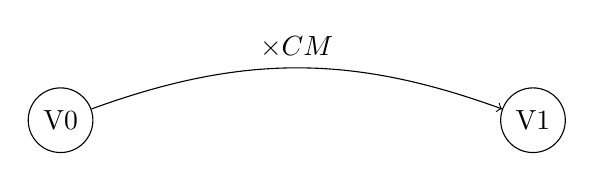
\begin{tikzpicture}[node distance=6cm]
	\tikzstyle{value} = [circle, draw]

	% Define nodes
	\node[value] (V1) {V1};
	\node[value] (V0) [left of=V1] {V0};
	
	% Draw edges with labels
	\draw[->, bend left=20] (V0) to node[midway, above] {$\times CM$} (V1);
		
	\end{tikzpicture}
\end{center}

\end{defi}

\begin{prop}{Calcul du coefficient multiplicateur}{}
On peut calculer le coefficient multiplicateur à partir du taux d'évolution. En effet, on a : $$CM = 1 + t$$
\end{prop}

\begin{ex}{}{}
Le prix d'un jeu vidéo, égal à $12$€, augmente de $3\%$. Calculer le coefficient multiplicateur $CM$ puis le prix $V_1$ après augmentation.
\begin{reponse}
	Le pourcentage d'augmentation est $p=3\%$.

	Le taux d'évolution est $t=0.03$.

	Le coefficient multiplicateur est $CM=1+t=1+0.03=1.03$.

	\begin{itemize}
		\item 
		\textbf{Première méthode :} Le prix final est donc $V_1 = CM\times V_0 =1.03\times 12 =12.36\text{€}$.
		\item 
		\textbf{Deuxième méthode :} L'augmentation de prix est $t\times V_0 = 0.03\times 12 =0.36\text{€}$.

		Le prix final est donc $V_1 = V_0 + t\times V_0 =12 +0.36 = 12.36\text{€}$.
	\end{itemize}



\end{reponse}
\end{ex}


\begin{prop}{Sens de variation}{}
Grâce au relation entre le coefficient multiplicateur $CM$ et le taux d'évolution $t$, on a :
\begin{itemize}
\item Si $CM > 1$, alors  on a \textbf{une augmentation}, $V_1>V_0$. 
\item Si $CM = 1$, alors il n'y a pas d'évolution, $V_0=V_1$. 
\item Si $CM < 1$, alors  on a \textbf{une diminution}, $V_1<V_0$.
\end{itemize}
\end{prop}

\section{Évolutions successives}

\begin{ex}{}{}
Le PEL (Plan d'Epargne Logement) permet de placer de l'argent au taux t de $2\%$ par an. Pierre a placé $1000$€ sur son PEL et il aimerait connaître le montant sur son compte au bout de 2 ans, puis de 5 ans.
\bigbreak

Afin de simplifier les calculs, dès que l'on travaille sur des évolutions successives, on travaillera toujours avec les \textbf{coefficients multiplicateurs}.
$$CM = \troum{1 + t  =  1 + \frac{2}{100} = 1 + 0.02 = 1.02} $$

Représentation de la situation au bout de deux ans :
\begin{center}
	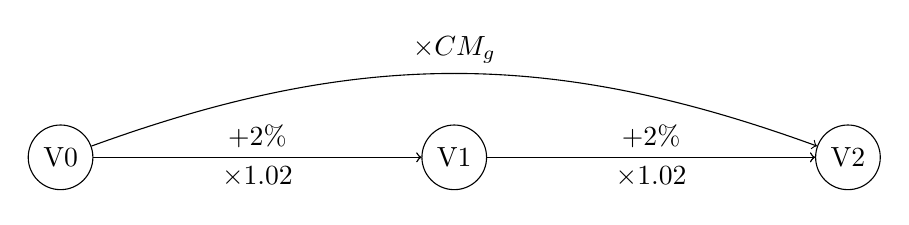
\begin{tikzpicture}[node distance=5cm]
		\tikzstyle{value} = [circle, draw]

		% Define nodes with circles
		\node[value] (V1) {V1};
		\node[value] (V0) [left of=V1] {V0};
		\node[value] (V2) [right of=V1] {V2};
		
		% Draw edges with plain text labels
		\draw[->] (V0) -- (V1) node[midway, below] {\normalsize$\times 1.02$};
		\draw[->] (V0) -- (V1) node[midway, above] {\normalsize$+2\%$};
		\draw[->] (V1) -- (V2) node[midway, below] {\normalsize$\times 1.02$};
		\draw[->] (V1) -- (V2) node[midway, above] {\normalsize$+2\%$};
		\draw[->, bend left=20] (V0) to node[midway, above] {\normalsize$\times CM_{g}$} (V2);
		
		\end{tikzpicture}
\end{center}

D'après les formules vu précédemment, on a :
\[V_{2} = V_{1}\times 1.02 \quad \text{ et } \quad V_{1} = V_{0}\times 1.02\]
Donc :
\begin{eqnarray*}
V_{2} &=& \textcolor{red}{V_{0}\times 1.02} \times 1.02\\
CM_{g} &=& \troum{\frac{V_{2}}{V_{0}} = 1.02^{2} \quad = \quad 1.0404}
\end{eqnarray*}

Une fois que l'on a obtenu le coefficient multiplicateur global $CM_{g}$ sur les deux années, on peut trouver le taux d'évolution globale :

$t_{g} = \troum{CM_{g} - 1  =  1.0404 - 1 = 0.0404}$ et \qquad $p=\troum{4.04 \%}$

\smallskip
Le taux d'évolution globale sur les deux ans est donc de $4.04\%$ \emph{(et pas de $4\%$ comme on aurait pu supposer)}

Finalement, Pierre aura sur son PEL $1040.4$€ au bout de deux ans.
\bigbreak

Représentation de la situation au bout de 5 ans :
\begin{center}
	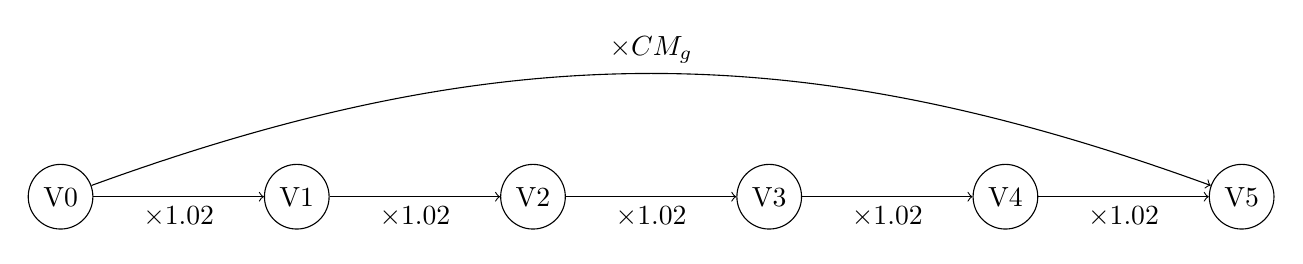
\begin{tikzpicture}[node distance=3cm]
	\tikzstyle{value} = [circle, draw]
	
	% Define nodes with circular style
	\node[value] (V1) {V1};
	\node[value] (V0) [left of=V1] {V0};
	\node[value] (V2) [right of=V1] {V2};
	\node[value] (V3) [right of=V2] {V3};
	\node[value] (V4) [right of=V3] {V4};
	\node[value] (V5) [right of=V4] {V5};
	
	% Draw straight edges with labels
	\draw[->] (V0) -- (V1) node[midway, below] {$\times 1.02$};
	\draw[->] (V1) -- (V2) node[midway, below] {$\times 1.02$};
	\draw[->] (V2) -- (V3) node[midway, below] {$\times 1.02$};
	\draw[->] (V3) -- (V4) node[midway, below] {$\times 1.02$};
	\draw[->] (V4) -- (V5) node[midway, below] {$\times 1.02$};
	
	% Curved edge from V0 to V5
	\draw[->, bend left=20] (V0) to node[midway, above] {$\times CM_{g}$} (V5);
	
	\end{tikzpicture}
\end{center}
	

En suivant le même raisonnement que pour deux ans, on obtient :

\[V_{2} = V_{0}\times 1.02\times 1.02\times 1.02\times 1.02\times 1.02\]

$$CM_{g} = \troum{ 1.02^{5} \quad \approx \quad 1.1041 } $$


Donc :

$t_{g} =\troum{CM_{g} - 1  \approx  1.1041 - 1 \approx 0.1041}$ et \qquad $p\approx\troum{10.41 \%}$

Le taux d'évolution globale sur les 5 ans est donc de $10.41\%$.

Finalement, Pierre aura sur son PEL $1104.1$€ au bout de 5 ans.
\end{ex}

\begin{prop}{Coefficient multiplicateur lors d'une évolution successive}{}
	Lors d'évolutions successives avec pour coefficients multiplicateurs $CM_1, CM_2, \dots, CM_n$, le coefficient multiplicateur global $CM_g$ est :

	\vspace{-3mm}
	$$CM_g = CM_1\times CM_2\times \dots\times CM_n$$

En particulier, si les coefficients multiplacteurs successifs sont égaux :
	
	$$CM_g = CM \times CM \times \dots\times CM = CM^n$$

\end{prop}
\newpage

\section{Évolutions réciproques}

\begin{ex}{}{}
Le cours du lait a perdu $20\%$ entre l'année 2009 et 2010. Les éleveurs français, en colère, demande au gouvernement une revalorisation de celui-ci afin de retrouver les cours de 2009. Le Ministre de l'Agriculture aimerait connaître le taux d'évolution que suggère d'appliquer les éleveurs avant d'en parler à son gouvernement.
Pouvez-vous l'aider ?
\bigbreak

Calcul du coefficient multiplicateur associé à une baisse de $20\%$

$$CM = \troum{1+t=1+\frac{-20}{100}=1-0.2=0.8}$$

\paragraph*{Schématisation du problème :}
\begin{center}
	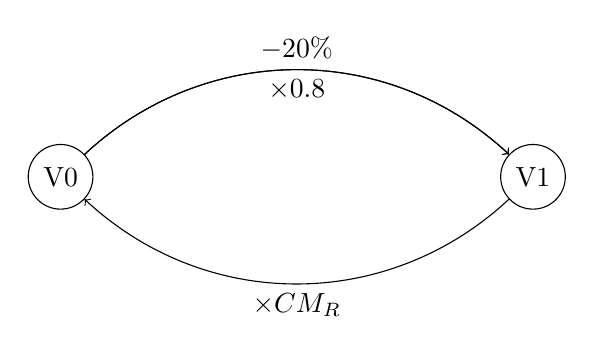
\begin{tikzpicture}[node distance=6cm]
	\tikzstyle{value} = [circle, draw]

	% Define nodes
	\node[value] (V1) {V1};
	\node[value] (V0) [left of=V1] {V0};
	
	% Draw edges with labels
	\draw[->, bend left=43] (V0) to node[midway, above] {$-20\%$} (V1);
	\draw[->, bend left=43] (V0) to node[midway, below] {$\times 0.8$} (V1);
	\draw[->, bend left=43] (V1) to node[midway, below] {$\times CM_{R}$} (V0);
		
	\end{tikzpicture}
\end{center}
	
D'après les formules vu précédemment, on a :
\[V_{1} = V_{0}\times 0.8 \text{ et }V_{0} = V_{1}\times CM_{R}\]
Donc :
\begin{eqnarray*}
V_{1} &=& \textcolor{red}{V_{1}\times CM_{R}}\times 0.8\\
1 &=& CM_{R}\times 0.8\\
\end{eqnarray*}

$$CM_R = \troum{\frac{1}{0.8} = 1.25}$$

On en déduit la valeur du taux d'évolution réciproque $t_{R}$ :
$$t_{R} =\troum{ CM_{R} - 1 = 1.25 - 1 = 0.25}$$

$$p=\troum{25\%}$$

Le Ministre de l'Agriculture devra donc demander que le cours du lait soit augmenté de $25\%$ pour que les éleveurs se retrouve dans la situation de 2009.
\end{ex}

\begin{prop}{Coefficient multiplicateur réciproque}{}
	Lors d'une évolution de coefficient multiplicateur $CM$, le coefficient multiplicateur réciproque $CM_R$ permettant de revenir à la situation initiale est :

	$$CM_R = \frac{1}{CM}$$

\end{prop}

\section*{Exercices}
\begin{exercicesnofoot}
	\sectionexo{Taux d'évolution et coefficient multiplicateur}
	\begin{bookexos}{54, 56 p.288}\end{bookexos}
	\begin{bookexo}{60 p.289}\end{bookexo}
	\sectionexo{Taux d'évolution successifs}
	\begin{bookexo}{69 p.290}\end{bookexo}
	\sectionexo{Taux d'évolution réciproque}
	\begin{bookexos}{70,72 p.290}\end{bookexos}
\end{exercicesnofoot}



\end{document}

